\documentclass[a4paper]{article}
\addtolength{\hoffset}
{-2.25cm}
\addtolength{\textwidth}
{5cm}
\addtolength{\voffset}
{-3.25cm}
\addtolength{\textheight}
{5.5cm}
\setlength{\parskip}{0pt}
\setlength{\parindent}{0in}

\usepackage[utf8]{inputenc}
\usepackage{microtype}
\usepackage[english]{babel}
\usepackage{fancyhdr}
\usepackage{advdate}
\usepackage{enumitem}
\usepackage{amsmath, amssymb}
\usepackage{graphicx}
\usepackage{caption}
\usepackage{subcaption}
\usepackage{float}
\usepackage{titlesec}
\usepackage{wasysym}
\usepackage{url}
\usepackage{hyperref}
\usepackage{tikz, verbatimbox}
\usepackage{fixltx2e}
\usepackage{centernot}
\usepackage{algorithm}
\usepackage{algpseudocode}
\usepackage{listings}
\usetikzlibrary{shapes.geometric, arrows}
\usetikzlibrary{positioning}
\usepackage[table]{xcolor}

\graphicspath{{./static/}}
\tikzset{every picture/.style={line width=0.75pt}} %set default line width to 0.75pt

\newcommand{\LComment}[1]{\State \(\triangleright\) \text{#1}}
\MakeRobust{\Call}

\begin{document}

\fancyhead[c]{}
\hrule \medskip
\begin{minipage}{0.195\textwidth}
\raggedright
Rishabh Indoria\\
21F3001823
\end{minipage}
\begin{minipage}{0.6\textwidth}
\centering
\LARGE
AI: Search Methods for Problem-Solving
\end{minipage}
\begin{minipage}{0.195\textwidth}
\raggedleft
\today \hfill \\
\end{minipage}
\medskip \hrule
\bigskip

\section{Introduction and History}

\subsection{Intelligent Agents}
\begin{itemize}
    \item \textbf{A First Course in Artificial Intelligence} by Deepak Khemani. First 7 chapters will be covered.
    \item \textbf{Intelligent Agents}: An entity that is persistent(it's there all the time), autonomous, proactive(decide what goals to achieve next) and goal directed(once it has goals, it will follow them). Human beings are also agents.
    \item An intelligent agent in a world carries a model of the world in its "head". the model may be an abstraction. A self-aware agent would model itself in the world model.
    \item Signal$\rightarrow$Symbol$\rightarrow$Signal
    \item Sense(Signal Processing) $\rightarrow$ Deliberate(Neuro fuzzy reasoning + Symbolic Reasoning) $\rightarrow$ Act(Output Signal)
    \begin{figure}[H]
        \centering
        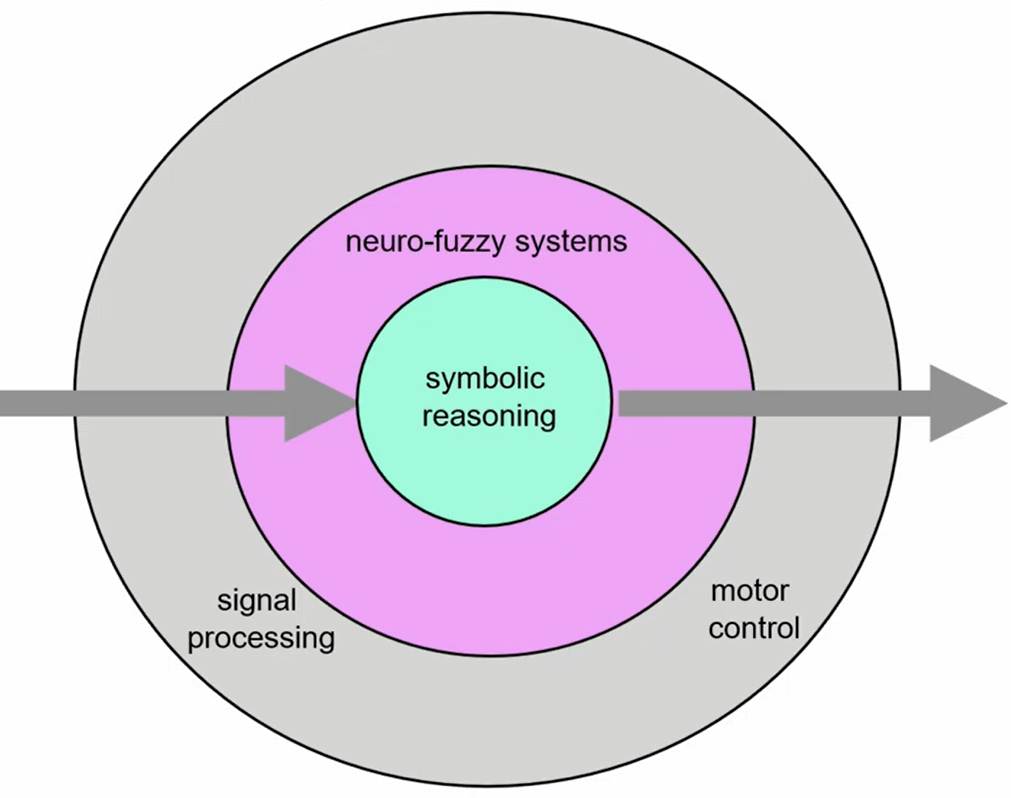
\includegraphics[width=0.5\linewidth]{Degree//static/AI_information_processing_view.png}
        \caption{Information Processing View of AI}
        \label{fig:AI-information-processing}
    \end{figure}
    \item \textbf{Intelligence}: \textbf{Remember the past and learn from it.} Memory and experience(case based reasoning), Learn a model(Machine learning), Recognize objects, faces, patterns(deep neural networks).\\
    \textbf{Understand the present. Be aware of the world around you.} Create a model of the world(knowledge representation), Make inferences from what you know(logic and reasoning).\\
    \textbf{Imagine the future. Work towards your goals.} Trial and error(heuristic search), Goals, plans, and actions(automated planning).
\end{itemize}

\subsection{Human Cognitive Architecture}
\begin{itemize}
    \item \textbf{Knowledge and Reasoning}: What does the agent know and what else does the agent know as a consequence of what it knows.
    \item \textbf{Semiotics}: A symbol is something that stands for something else. All languages, both spoken and written, are semiotic systems.
    \item \textbf{Biosemiotics}: How complex behaviour emerges when simple systems interact with each other through signs.
    \item \textbf{Reasoning}: The manipulation of symbols in a meaningful manner.
\end{itemize}

\subsection{Problem-Solving}
\begin{itemize}
    \item An autonomous agent in some world has a goal to achieve and a set of actions to choose from to strive for the goal.
    \item We deal with simple problems first, i.e., the world is static, the world is completely known, only one agent changes the world, action never fail, representation of the world is taken care of.
\end{itemize}

\section{Search Methods}

\subsection{State Space Search}
\begin{itemize}
    \item We start with the map coloring problem, where we want to color each region in the map with an allowed color such that no two adjacent regions have the same color.
    \begin{figure}[H]
        \centering
        \begin{subfigure}[b]{0.45\textwidth}
            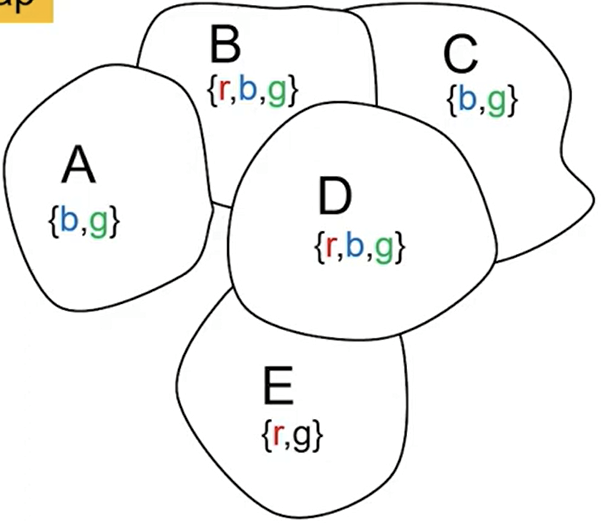
\includegraphics[width=1\textwidth]{Degree/static/AI_map_colors.png}
            \caption{Map with Constraints}
            \label{fig:AI-map-constraint}
        \end{subfigure}
        \hfill
        \begin{subfigure}[b]{0.45\textwidth}
            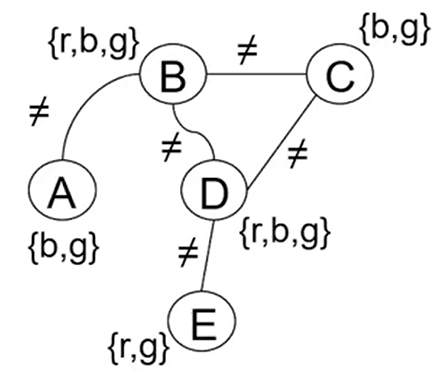
\includegraphics[width=1\textwidth]{Degree/static/AI_constraint_graph.png}
            \caption{Constraint Graph}
            \label{fig:AI-constraint-graph}
        \end{subfigure}
        \caption{Map Coloring Problem}
        \label{fig:AI-map-coloring-problem}
    \end{figure}
    \textbf{Brute Force}: Try all combinations of color for all regions.\\
    \textbf{Informed Search}: Choose a color that does not conflict with neighbors.\\
    \textbf{General Search}: Pose the problem to serve as an input to a general search algorithm.\\
    Map coloring can be posed as a constraint satisfaction problem or as a state space search, where the move is to assign a color to a region in a given partially colored state.
    \item \textbf{General Purpose methods}: Instead of writing a custom program for every problem to be solved, these aim to write search algorithms into which individual methods can be plugged in. One of them is State Space Search.
    \item \textbf{State or Solution Space Search}: Describe the given state, devise an operator to choose an action in each state, and then navigate the state space in search of the desired or goal state. Also known as Graph Search.\\
    A \textbf{state} is a representation of a situation.\\
    A \textit{MoveGen} function captures the moves that can be made in a given state.\\
    It returns a set of states - \textit{neighbors} - resulting from the moves.\\
    The state space is an implicit graph defined by the \textit{MoveGen} function.\\
    A \textit{GoalTest} function checks if the given state is a \textit{goal} state.\\
    A \textit{search algorithm} navigates the state space using these two functions.
    \item \textbf{The Water Jug Problem}: You have three jugs with capacity 8, 5 and 3 liters. Any state can be written as $[a,b,c]$, where $a,b,c$ are the amount of water present in each jug\\
    Start state: The 8-liter jug is filled with water, and the other two are empty, $[8,0,0]$. It can be seen that at any state the total amount of water remains the same.\\
    Goal: You are required to measure 4 liters of water. So, our goal state is $[4,x,y]$ or $[x,4,y]$ or $[x,y,4]$. A \textit{GoalTest} function can be written as
    \begin{algorithm}[H]
    \caption{GoalTest for the Water Jug Problem}\label{alg:AI-goal-test-water-jug}
        \begin{algorithmic}[1]
            \Require $[a,b,c]$, the state which needs to be checked
            \If{$a=4$ or $b=4$ or $c=4$}
                \State \Return True
            \EndIf
            \State \Return False
        \end{algorithmic}
    \end{algorithm}
    \item A few other examples are \textbf{The Eight Puzzle}, \textbf{The Man, Goat, Lion, Cabbage} and \textbf{The N-Queens Problem}.
\end{itemize}
Before studying different algorithms, we need to familiarize ourselves with some pseudocode syntax.

\pagebreak
\setlength{\voffset}{0cm}
\setlength{\hoffset}{0cm}
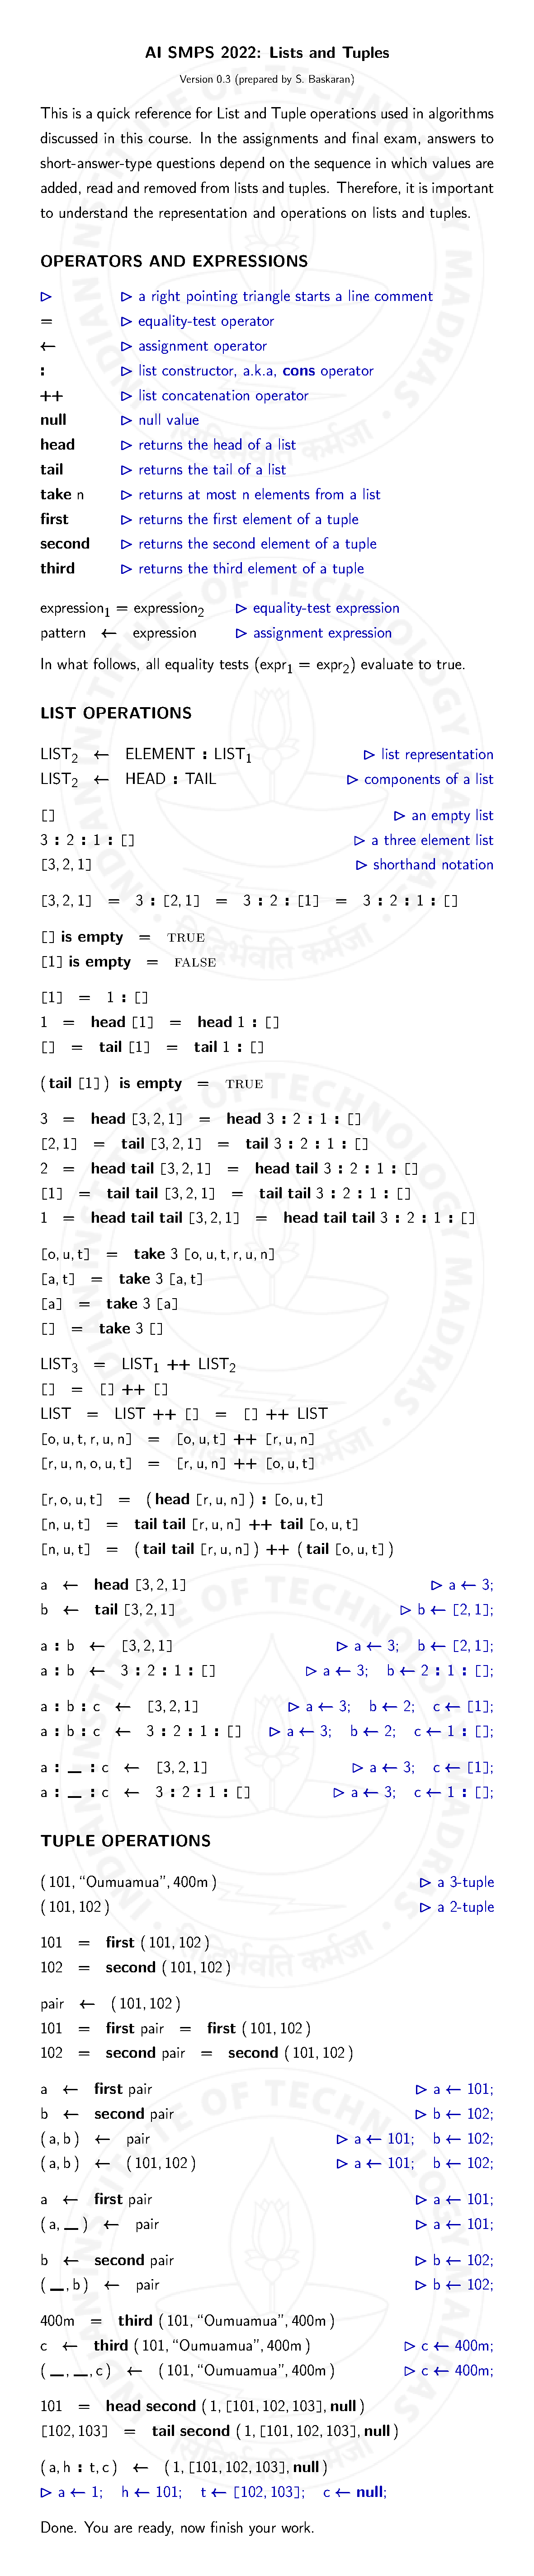
\includepdf[pages={1}, trim=0 71cm 0 0, clip]{AI_reference.pdf}
\setlength{\voffset}{\originalVOffset}
\setlength{\hoffset}{\originalHOffset}
\pagebreak
\setlength{\voffset}{0cm}
\setlength{\hoffset}{0cm}
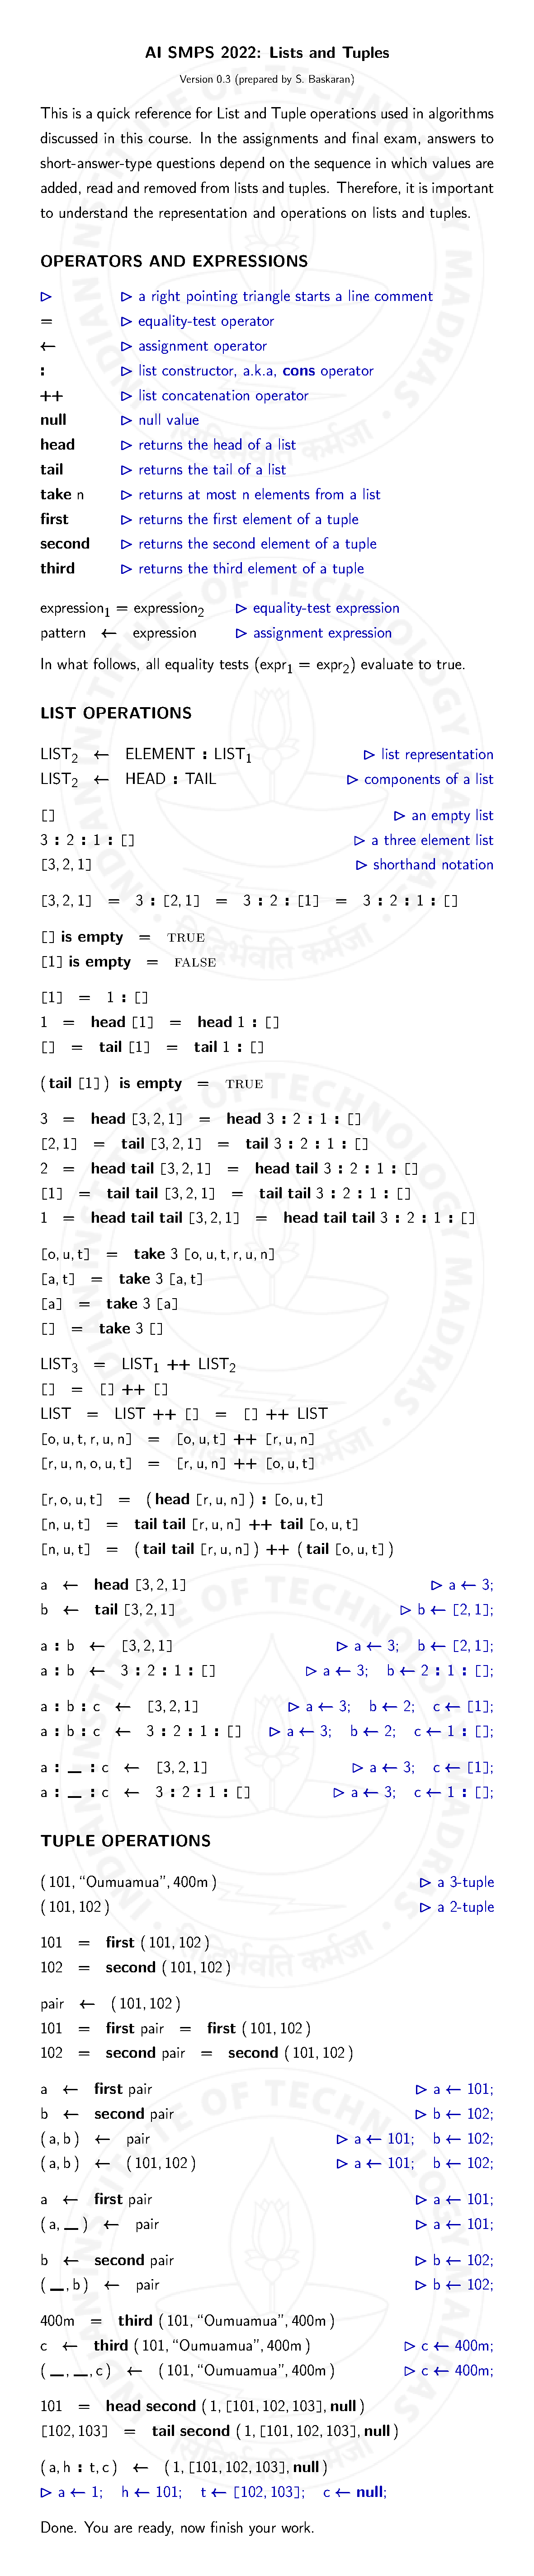
\includepdf[pages={1}, trim=0 45cm 0 26cm, clip]{AI_reference.pdf}
\setlength{\voffset}{\originalVOffset}
\setlength{\hoffset}{\originalHOffset}
\pagebreak
\setlength{\voffset}{0cm}
\setlength{\hoffset}{0cm}
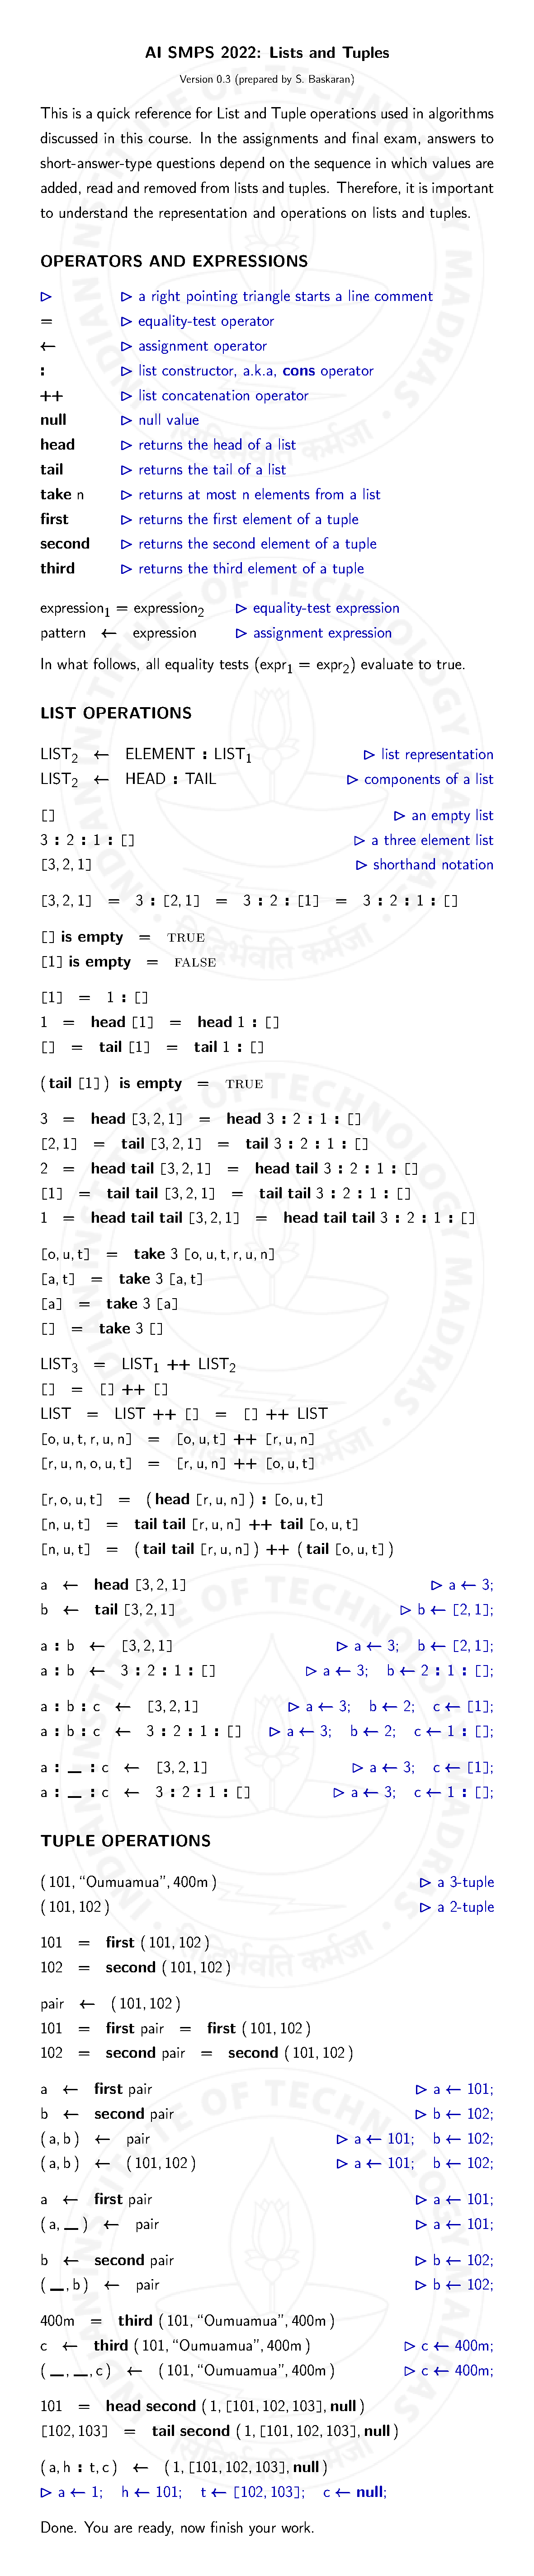
\includepdf[pages={1}, trim=0 20cm 0 50.5cm, clip]{AI_reference.pdf}
\setlength{\voffset}{\originalVOffset}
\setlength{\hoffset}{\originalHOffset}
\pagebreak
\setlength{\voffset}{0cm}
\setlength{\hoffset}{0cm}
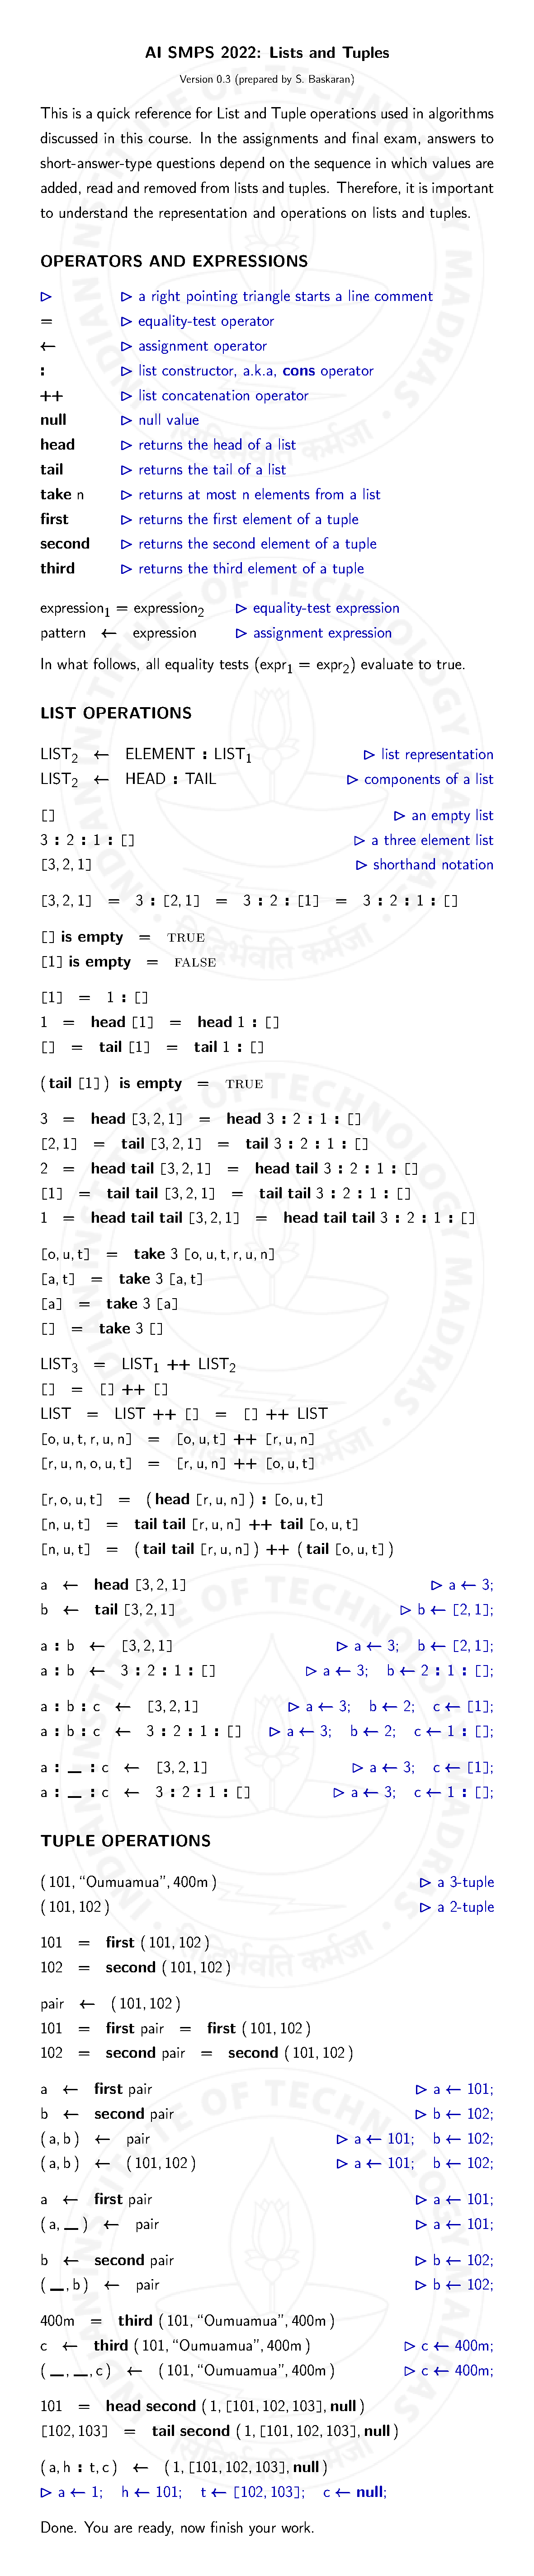
\includepdf[pages={1}, trim=0 0 0 76.5cm, clip]{AI_reference.pdf}
\setlength{\voffset}{\originalVOffset}
\setlength{\hoffset}{\originalHOffset}
\pagebreak

\subsection{General Search Algorithms}
\begin{itemize}
    \item Searching is like treasure hunting. Our approach would be to generate and test where we traverse the space by generating new nodes and test each node whether it is the goal or not.
    \item \textbf{Simple Search 1}: Simply pick a node N from OPEN and check if it is the goal.
    \begin{algorithm}[H]
        \caption{Simple Search 1}\label{alg:AI-simple-search-1}
        \begin{algorithmic}[1]
            \LComment{S is the initial state}
            \State OPEN $\gets \{S\}$
            \While{\textit{OPEN} is not empty}
                \State pick some node N from OPEN
                \State OPEN $\gets$ OPEN - $\{n\}$
                \If{\Call{GoalTest}{N} = True}
                    \State \Return N
                \Else
                    \State OPEN $\gets$ OPEN $\cup$ \Call{MoveGen}{N}
                \EndIf
            \EndWhile
            \State \Return FAILURE
        \end{algorithmic}
    \end{algorithm}
    This algorithm may run into an infinite loop, to address it we have \textbf{Simple Search 2}.
    \begin{algorithm}[H]
        \caption{Simple Search 2}\label{alg:AI-simple-search-2}
        \begin{algorithmic}[1]
            \LComment{S is the initial state}
            \State OPEN $\gets \{S\}$
            \State CLOSED $\gets \{\}$ 
            \While{\textit{OPEN} is not empty}
                \State pick some node N from OPEN
                \State OPEN $\gets$ OPEN - $\{n\}$
                \State CLOSED $\gets$ CLOSED $\cup$ $\{N\}$
                \If{\Call{GoalTest}{N} = True}
                    \State \Return N
                \Else
                    \State OPEN $\gets$ OPEN $\cup$ $\{$\Call{MoveGen}{N} - CLOSED$\}$
                \EndIf
            \EndWhile
            \State \Return FAILURE
        \end{algorithmic}
    \end{algorithm}
    We can modify this a bit further by doing, OPEN $\gets$ OPEN $\cup$ $\{$\textit{MoveGen(N)} - CLOSED - OPEN$\}$, this lowers the state space even more.
\end{itemize}

\subsection{Planning and Configuration Problems}
\begin{itemize}
    \item \textbf{Planning Problems}: Goal is known or describe, path is sought. Examples include River crossing problems, route finding etc.
    \item \textbf{Configuration Problems}: A state satisfying a description is sought. Examples include N-queens, crossword puzzle, Sudoku, etc.
    \item The simple search algorithms will work for configuration problems, but they won't return any path.
    \item \textbf{NodePairs}: Keep track of parent nodes. Each node is a pair $(currentNode,\text{ }parentNode)$.
    \item \textbf{Depth First Search}: OPEN is a stack data structure
    \begin{algorithm}[H]
        \caption{Depth First Search}\label{alg:AI-DFS}
        \begin{algorithmic}[1]
            \State OPEN $\gets$ (S, null) : [ ]
            \State CLOSED $\gets$ [ ]
            \While{OPEN is not empty}
                \State nodePair $\gets$ head OPEN
                \State (N, $\_$) $\gets$ nodePair
                \If{\Call{GoalTest}{N} = True}
                    \State \Return \Call{ReconstructPath}{nodePair, CLOSED}
                \EndIf
                \State CLOSED $\gets$ nodePair : CLOSED
                \State children $\gets$ \Call{MoveGen}{N}
                \State newNodes $\gets$ \Call{RemoveSeen}{children, OPEN, CLOSED}
                \State newPairs $\gets$ \Call{MakePairs}{newNodes, N}
                \State OPEN $\gets$ newPairs ++ tail OPEN
            \EndWhile
            \State \Return [ ]
            \Statex
            \Function{RemoveSeen}{nodeList, OPEN, CLOSED}
                \If{nodeList = [ ]}
                    \State \Return [ ]
                \EndIf
                \State node $\gets$ head nodeList
                \If{\Call{OccursIn}{node, OPEN} or \Call{OccursIn}{node, CLOSED}}
                    \State \Return \Call{RemoveSeen}{tail nodeList, OPEN, CLOSED}
                \EndIf
                \State \Return node : \Call{RemoveSeen}{tail nodeList, OPEN, CLOSED}
            \EndFunction
            \Statex
            \Function{OccursIn}{node, nodePairs}
                \If{nodePairs = [ ]}
                    \State \Return FALSE
                \ElsIf{node = first head nodePairs}
                    \State \Return TRUE
                \EndIf
                \State \Return \Call{OccursIn}{node, tail nodePairs}
            \EndFunction
            \Statex
            \Function{MakePairs}{nodeList, parent}
                \If{nodeList = [ ]}
                    \State \Return [ ]
                \EndIf
                \State \Return (head nodeList, parent) : \Call{MakePairs}{tail nodeList, parent}
            \EndFunction
            \Statex
            \Function{ReconstructPath}{nodePair, CLOSED}
                \State (node, parent) $\gets$ nodePair
                \State path $\gets$ node : [ ]
                \While{parent is not null}
                    \State path $\gets$ parent : path
                    \State CLOSED $\gets$ \Call{SkipTo}{parent, CLOSED}
                    \State($\_$, parent) $\gets$ head CLOSED
                \EndWhile
                \State \Return path
            \EndFunction
            \algstore{bkbreak}
        \end{algorithmic}
    \end{algorithm}
    \begin{algorithm}[H]
        \caption{Depth First Search continued}
        \begin{algorithmic}
            \algrestore{bkbreak}
            \Statex
            \Function{SkipTo}{parent, nodePairs}
                \If{parent = first head nodePairs}
                    \State \Return nodePairs
                \EndIf
                \State \Return \Call{SkipTo}{parent, tail nodePairs}
            \EndFunction
        \end{algorithmic}
    \end{algorithm}
    \item \textbf{Breadth First Search}: We use a queue for the OPEN set.
    \begin{algorithm}
        \caption{Breadth First Search}\label{alg:AI-BFS}
        \begin{algorithmic}
            \State OPEN $\gets$ (S, null) : [ ]
            \State CLOSED $\gets$ [ ]
            \While{OPEN is not empty}
                \State nodePair $\gets$ head OPEN
                \State (N, $\_$) $\gets$ nodePair
                \If{\Call{GoalTest}{N} = True}
                    \State \Return \Call{ReconstructPath}{nodePair, CLOSED}
                \EndIf
                \State CLOSED $\gets$ nodePair : CLOSED
                \State children $\gets$ \Call{MoveGen}{N}
                \State newNodes $\gets$ \Call{RemoveSeen}{children, OPEN, CLOSED}
                \State newPairs $\gets$ \Call{MakePairs}{newNodes, N}
                \LComment{This is the only line that is different, we now add newPairs at the end of the list}
                \State OPEN $\gets$ tail OPEN ++ newPairs 
            \EndWhile
            \State \Return [ ]
        \end{algorithmic}
    \end{algorithm}
    \item BFS always generates the shortest path, whereas DFS may not generate the shortest path.
    \item \textbf{Time Complexity}: Assume constant branching factor $b$ and assume the goal occurs somewhere at depth $d$. In the best case the goal would be the first node scanned at depth $d$ and in the worst case the goal would b3 the last node scanned.\\
    Best Case: $N_{DFS}=d+1$ and $N_{BFS}=\frac{b^{d}-1}{b-1}+1$\\
    Worst Case: $N_{DFS}=N_{BFS}=\frac{b^{d+1}-1}{b-1}$\\
    Average: $N_{DFS}\approx \frac{b^d}{2}$ and $N_{BFS}\approx \frac{b^d(b+1)}{2(b-1)}$, $N_{BFS}\approx N_{DFS}(\frac{b+1}{b-1})$
    \begin{table}[H]
        \centering
        \begin{tabular}{|c|c|c|}
            \hline
             & Depth First Search & Breadth First Search \\
             \hline
            Time & Exponential & Exponential\\
            \hline
            Space & Linear & Exponential\\
            \hline
            Quality of Solution & No guarantees & Shortest path\\
            \hline
            Completeness & Not for infinite search space & Guaranteed to terminate if solution path exists\\
            \hline
        \end{tabular}
        \caption{DFS vs BFS}
        \label{tab:AI-DFS-vs-BFS}
    \end{table}
    \item \textbf{Depth Bounded DFS}: Do DFS with a depth bound $d$. It is not complete and does not guarantee the shortest path. Given below is a modified version that returns the count of nodes visited, to get the original version just remove count.
    \begin{algorithm}[H]
        \caption{Depth Bounded DFS}\label{alg:AI-depth-DFS}
        \begin{algorithmic}[1]
            \State count $\gets$ 0
            \State OPEN $\gets$ (S, null, 0) : [ ]
            \State CLOSED $\gets$ [ ]
            \While{OPEN is not empty}
                \State nodePair $\gets$ head OPEN
                \State (N, $\_$, depth) $\gets$ nodePair
                \If{\Call{GoalTest}{N} = True}
                    \State \Return count, \Call{ReconstructPath}{nodePair, CLOSED}
                \EndIf
                \State CLOSED $\gets$ nodePair : CLOSED
                \If{depth $<$ depthBound}
                    \State children $\gets$ \Call{MoveGen}{N}
                    \State newNodes $\gets$ \Call{RemoveSeen}{children, OPEN, CLOSED}
                    \State newPairs $\gets$ \Call{MakePairs}{newNodes, N, depth + 1}
                    \State OPEN $\gets$ newPairs ++ tail OPEN
                    \State count $\gets$ count + length newPairs
                \Else
                    \State OPEN $\gets$ tail OPEN
                \EndIf
            \EndWhile
            \State \Return count, [ ]
        \end{algorithmic}
    \end{algorithm}
    \item \textbf{Depth First Iterative Deepening}: Iteratively increase depth bound. Combines best of BFS and DFS. This will give the shortest path, but we have to be careful that we take correct nodes from CLOSED. $N_{DFID}\approx N_{BFD}\frac{b}{b-1}$ for large $b$.
    \begin{algorithm}[H]
        \caption{Depth First Iterative Deepening}\label{alg:AI-depth-first-iterative}
        \begin{algorithmic}[1]
            \State count $\gets$ $-1$
            \State path $\gets$ [ ]
            \State depthBound $\gets$ $0$
            \Repeat
                \State previousCount $\gets$ count
                \State (count, path) $\gets$ \Call{DB-DFS}{$S,depthBound$}
                \State depthBound $\gets$ depthBound $+1$
            \Until{(path is not empty) or (previousCount $==$ count)}
            \State \Return path
        \end{algorithmic}
    \end{algorithm}
    \item DFID-C as compared to regular DFID-N adds new neighbors to OPEN list and also adds neighbors that are in CLOSED but not in OPEN list. This allows DFID-C to get the shortest path whereas DFID-N may not get the shortest path.
    \item The monster that AI fights is Combinatorial Explosion.
    \item All these algorithms we studied are blind algorithms or uniformed search, they don't know where the goal is.
\end{itemize}

\subsection{Heuristic Search}
\begin{itemize}
    \item Testing the neighborhood and following the steepest gradient identifies which neighbors are the lowest or closest to the bottom.
    \item The heuristic function $h(N)$ is typically a user defined function, $h(Goal)=0$.
    \item \textbf{Best First Search}: Instead of having a simple stack or queue we use a priority queue sorted based on heuristic function. Search frontier depends upon the heuristic function. If graph is finite then this is complete and quality of solution will head towards the goal but may not give the shortest path.
    \begin{algorithm}[H]
        \caption{Best First Search}\label{alg:AI-BestFS}
        \begin{algorithmic}[1]
            \State OPEN $\gets$ (S, null, h(S)) : [ ]
            \State CLOSED $\gets$ [ ]
            \While{OPEN is not empty}
                \State nodePair $\gets$ head OPEN
                \State (N, $\_$, $\_$) $\gets$ nodePair
                \If{\Call{GoalTest}{N} = True}
                    \State \Return \Call{ReconstructPath}{nodePair, CLOSED}
                \EndIf
                \State CLOSED $\gets$ nodePair : CLOSED
                \State children $\gets$ \Call{MoveGen}{N}
                \State newNodes $\gets$ \Call{RemoveSeen}{children, OPEN, CLOSED}
                \State newPairs $\gets$ \Call{MakePairs}{newNodes, N}
                \LComment{Again, this is pretty much the most important line}
                \State OPEN $\gets$ sort$_h$(newPairs ++ tail OPEN)
            \EndWhile
            \State \Return [ ]
        \end{algorithmic}
    \end{algorithm}
    \item For The eight puzzle we can define a few heuristic functions as follows:\\
    $h_1(n)=$ number of tiles out of place, Hamming distance.\\
    $h_2(n)=$ $\sum_{\text{for each tile}}$ Manhattan distance to its destination.
    \item \textbf{Hill Climbing}: A local search algorithm, i.e., move to the best neighbor if it is better, else terminate. In practice sorting is not needed, only the best node. This has burnt its bridges by not storing OPEN. We are interested in this because it is a constant space algorithm, which is a vast improvement on the exponential space for BFS and DFS. It's time complexity is linear. It treats the problem as an optimization problem.
    \begin{algorithm}[H]
        \caption{Hill Climbing}\label{alg:AI-hill-climbing}
        \begin{algorithmic}[1]
            \State node $\gets$ Start
            \State newNode $\gets$ head(sort$_h$(moveGen(node)))
            \While{ $h(newNode)<$ $h(node)$}
                \State node $\gets$ newNode
                \State newNode $\gets$ head(sort$_h$(moveGen(node)))
            \EndWhile
            \State \Return node
        \end{algorithmic}
    \end{algorithm}
\end{itemize}

\subsection{Escaping Local Optima}
\begin{itemize}
    \item \textbf{Solution Space Search}: Formulation of the search problem such that when we find the goal node we have the solution, and we are done.
    \item \textbf{Synthesis Methods}: Constructive methods. Starting with the initial state and build the solution state piece by piece.
    \item \textbf{Perturbation Methods}: Permutation of all possible candidate solutions.
    \item \textbf{SAT problem}: Given a boolean formula made up of a set of propositional variables $V=\{a,b,c,d,e,...\}$ each of which can be $true$ or $false$, or $1$ or $0$, to find an assignment of variables such that the given formula evaluates to $true$ or $1$.\\
    A SAT problem with $N$ variables has $2^N$ candidates.
    \item \textbf{Travelling Salesman Problem}: Given a set of cities and given a distance measure between every pair of cities, the task is to find a Hamiltonian cycle, visiting each city exactly once, having the least cost.
    \begin{enumerate}
        \item \textbf{Nearest Neighbor Heuristic}: Start at some city, move to nearest neighbor as long as it does not close the loop prematurely.
        \item \textbf{Greedy Heuristic}: Sort the edges, then add the shortest available edge to the tour as long as it does not close the loop prematurely.
        \item \textbf{Savings Heuristic}: Start with $n-1$ tours of length $2$ anchored on a base vertex and performs $n-2$ merge operations to construct the tour.
        \item \textbf{Perturbation operators}: Start with some tour, then choose two cities and interchange, this gives the solution space. Heuristic function is $saving$ = $cost(base,a)$ + $cost(base,b)$ - $cost(a,b)$
        \item \textbf{Edge Exchange}: Similar to above but now instead of choosing cities we are choosing edges. Can be $2$-edge exchange, $3$-edge, $4$-edge, etc. City exchange is a special case of $4$-edge exchange.
    \end{enumerate}
    \item Solution space of TSP grows in order factorial, much faster than SAT problem.
    \item A collection of problems with some solutions is available \href{http://comopt.ifi.uni-heidelberg.de/software/TSPLIB95/}{here}.
    \item To escape local minima we need something called \textbf{exploration}.
    \item \textbf{Beam Search}: Look at more than one option at each level. For a beam width $b$, look at best $b$ options. Heavily memory dependent.
    \begin{algorithm}
        \caption{Beam Search}\label{alg:Beam-Search}
        \begin{algorithmic}
            \Statex \Call{BeamSearch}{$S,w$}
            \State OPEN $\gets$ $[S]$
            \State $N$ $\gets$ $S$
            \Do
                \State $bestEver$ $\gets$ $N$
                \If{\Call{Goal-Test}{OPEN} = True}
                    \State \Return goal from OPEN
                \EndIf
                \State $neighbors$ $\gets$ \Call{MoveGen}{OPEN}
                \State OPEN $\gets$ take w $sort_h(neighbors)$
                \State $N$ $\gets$ head(OPEN)
            \doWhile{$h(N)$ is better than $h(bestEver)$}
            \State \Return $bestEver$
        \end{algorithmic}
    \end{algorithm}
    \item \textbf{Variable Neighborhood Descent}: Essentially we are doing hill climbing with different neighborhood functions. The idea is to use sparse functions before using denser functions, so the storage is not high. The algorithm assumes that there are $N$ $moveGen$ functions sorted according to the density of the neighborhoods produced.
    \begin{algorithm}[H]
        \caption{Variable Neighborhood Descent}\label{alg:Variable-Neighborhood-Descent}
        \begin{algorithmic}[1]
            \Statex \Call{VariableNeighbourhoodDescent}{ }
            \State $node\gets$ $start$
            \For{$i\gets$ $1$ to $n$}
                \State $moveGen\gets$ \Call{MoveGen}{$i$}
                \State $node\gets$ \Call{HillClimbing}{$node,moveGen$}
            \EndFor
            \State \Return $node$
        \end{algorithmic}
    \end{algorithm}
    \item \textbf{Best Neighbor}: Another variation of Hill Climbing, simply move to the best neighbor regardless of whether it is better than current node or not. This will require an external criterion to terminate. It will not escape local maxima, as once it escapes it will go right back to it in the next iteration.
    \begin{algorithm}[H]
        \caption{Best Neighbor}\label{alg:best-neighbor}
        \begin{algorithmic}[1]
            \Statex \Call{BestNeighbor}{ }
            \State $N\gets$ $start$
            \State $bestSeen\gets$ $N$
            \While{some termination criterion}
                \State $N\gets$ \Call{best}{$moveGen(N)$}
                \If{$N$ better than $bestSeen$}
                    \State $bestSeen\gets$ $N$
                \EndIf
            \EndWhile
            \State \Return $bestSeen$
        \end{algorithmic}
    \end{algorithm}
    \item \textbf{Tabu Search}: Similar to Best Neighbor but not allowed back immediately. An aspiration criterion can be added that says that if a tabu move result in a node that is better than bestSeen then it is allowed. To drive this search into newer areas, keep a frequency array and give preference to lower frequency bits or bits that have been changed less.
    \begin{algorithm}[H]
        \caption{Tabu Search}\label{alg:tabu-search}
        \begin{algorithmic}[1]
            \Statex \Call{TabuSearch}{ }
            \State $N\gets$ $start$
            \State $bestSeen\gets$ $N$
            \While{some termination criterion}
                \State $N\gets$ \Call{best}{\Call{allowed}{$moveGen(N)$}}
                \If{$N$ better than $bestSeen$}
                    \State $bestSeen\gets$ $N$
                \EndIf
            \EndWhile
            \State \Return $bestSeen$
        \end{algorithmic}
    \end{algorithm}
\end{itemize}

\section{Stochastic Search}
Very often to escape local minima we use Stochastic/Randomized methods instead of Deterministic methods.
\subsection{Iterated Hill Climbing}
\begin{itemize}
    \item \textbf{2SAT}: Problems where each clause has at most two literals, known to be solved in polynomial time. However, if we add even 1 more literal it would become NP-complete or exponential.
    \item Iterated hill climbing says that we should perform hill climbing with multiple different starting nodes chosen randomly to have a higher probability of finding the goal node.
    \begin{algorithm}[H]
        \caption{Iterated Hill Climbing}\label{alg:AI-iterated-hill-climbing}
        \begin{algorithmic}[1]
            \Statex \Call{Iterated-Hill-Climbing}{$N$}
            \State $bestNode$ $\gets$ \textbf{random candidate solution}
            \For{$i\gets$ $1$ to $N$}
                \State $currentBest$ $\gets$ \Call{Hill-Climbing}{\textbf{new random candidate solution}}
                \If{$h(currentBest)$ is better than $h(bestNode)$}
                    \State $bestNode$ $\gets$ $currentBest$
                \EndIf
            \EndFor
            \State \Return $bestNode$
        \end{algorithmic}
    \end{algorithm}
\end{itemize}

\subsection{Stochastic Actions}
\begin{itemize}
    \item To move or not to move is the question.
    \item Idea is we would like to consider actions that are good in terms of heuristic functions, but sometimes we even want to move when heuristic function is not necessarily good.
    \item \textbf{Random Walk}: Choose a random node and move there, hill climbing of stochastic search.
    \begin{algorithm}[H]
        \caption{Random Walk}\label{alg:AI-random-walk}
        \begin{algorithmic}[1]
            \Statex \Call{RandomWalk}{ }
            \State $node$ $\gets$ random candidate solution or start
            \State $bestNode$ $\gets$ $node$
            \For{$i\gets$ $1$ to $n$}
                \State $node$ $\gets$ \Call{RandomChoose}{\Call{MoveGen}{$node$}}
                \If{$node$ is better than $bestNode$}
                    \State $bestNode$ = $node$
                \EndIf
            \EndFor
        \end{algorithmic}
    \end{algorithm}
    \item \textbf{Stochastic Hill Climbing}: Let the algorithm be at the current bode $v_c$, then we select a random neighbor $v_N$ and calculate $\Delta E=(eval(v_N)-eval(v_c))$.\\
    If $\Delta E$ is positive, it means that $v_N$ is better than $v_c$, then the algorithm should move to it with a higher probability.\\
    If $\Delta E$ is negative, it means that $v_N$ is better than $v_c$, then the algorithm should move to it with a lower probability.\\
    The probability is computed using the sigmoid function, which is given as
    \begin{equation*}
        \text{Probability }P=\frac{1}{1+e^{-\frac{\Delta E}{T}}}
    \end{equation*}
    where $T$ is a parameter. The algorithm essentially combines exploration with exploitation.
    \item \textbf{Annealing}: In metallurgy and materials science, \textbf{annealing} is a heat treatment that alters the physical and sometimes chemical properties of a material to increase its ductility and reduce its hardness, making it more workable. It involves heating a material above its recrystallization temperature, maintaining a suitable temperature for an appropriate amount of time and then cooling.\\
    In annealing, atoms migrate in the crystal lattice and the number of dislocations decreases, leading to a change in ductility and hardness. As the material cools it recrystallizes.
    \item \textbf{Simulated Annealing}: Essentially tries to mimic the annealing process, begins with exploration and ends with exploitation. Annealing is also where $\Delta E$ and $T$ come from, essentially meaning Energy and Temperature.
    \begin{algorithm}[H]
        \caption{Simulated Annealing}\label{alg:simulated-annealing}
        \begin{algorithmic}[1]
            \Statex \Call{SimulatedAnnealing}{ }
            \State $node\gets$ random candidate solution or start
            \State $bestNode\gets$ $node$
            \State $T\gets$ some large value
            \For{$time\gets$ $1$ to $numberOfEpochs$}
                \While{some termination criteria} \Comment{$M$ cycles in a sample case}
                    \State $neighbor\gets$ \Call{RandomNeighbor}{$node$}
                    \State $\Delta E\gets$ $Eval(neighbor)-Eval(node)$
                    \If{$Random(0,1)<$ \Call{Sigmoid}{$\Delta E, T$}}
                        \State $node\gets$ $neighbor$
                        \If{$Eval(node)>Eval(bestNode)$}
                            \State $bestNode\gets$ $node$
                        \EndIf
                    \EndIf
                \EndWhile
                \State $T\gets$ \Call{CoolingFunction}{$T,times$}
            \EndFor
            \State \Return $bestNode$
        \end{algorithmic}
    \end{algorithm}
\end{itemize}

\subsection{Genetic Algorithms}
\begin{itemize}
    \item Survival of the fittest. Inspired by the process of natural selection.
    \item A class of methods for optimization problems, more generally known as Evolutionary Algorithms.
    \item Implemented on a population of candidates in the solution space. A fitness function evaluates each candidate. The fittest candidates get to mate and reproduce.
    \item \textbf{Artificial Selection}: Given a population of candidate solutions we do a three step iterative process
    \begin{enumerate}
        \item \textbf{Reproduction}: Clone each candidate in proportion to its fitness. Some may get more than one copy, some none.
        \item \textbf{Crossover}: Randomly mate the resulting population and mix up the genes.
        \item \textbf{Mutation}: Once in a while, in search of a missing gene.
    \end{enumerate}
    \item \textbf{Selection}: Imagine a roulette wheel on which each candidate in the parent population $\{P_1,P_2,...,P_N\}$ is represented as a sector. The angle subtended by each candidate is proportional to its fitness. The roulette wheel is spun $N$ times. Then the selected parents are added one by one to create a new population.
    \item \textbf{Crossover Operators}: A \textit{single point crossover} simply cuts the two parents at a randomly chosen point and recombines them to form two new solution strings. It can be at multiple points as well, idea is to mix up the genes.
    \begin{algorithm}[H]
        \caption{Genetic Algorithm}\label{alg:genetic-algorithm}
        \begin{algorithmic}[1]
            \Statex \Call{Genetic-Algorithm}{ }
            \State $P\gets$ create $N$ candidate solutions \Comment{initial population}
            \Repeat
                \State compute fitness value for each member of $P$
                \State $S\gets$ with probability proportional to fitness value, randomly select $N$ member from $P$.
                \State $offspring\gets$ partition $S$ into two halves, and randomly mate and crossover members to generate $N$ offsprings.
                \State With a low probability mutate some offsprings
                \State Replace $k$ the weakest members of $P$ with $k$ strongest offsprings
            \Until{some termination criteria}
            \State \Return the best member of $P$
        \end{algorithmic}
    \end{algorithm}
    \item A large diverse population size is necessary for the performance of genetic algorithm to work.
    \item One issue is how to represent candidate solutions?, as they can be of any type. One simple solution is to convert the solution into a string this will require an additional function.
    \item In TSP, one problem is also that during crossover some cities can get repeated.
    \item \textbf{Cycle Crossover}: Identify cycles, look at below image, easier to understand.
    \begin{figure}[H]
        \centering
        \begin{subfigure}[b]{0.45\textwidth}
            \centering
            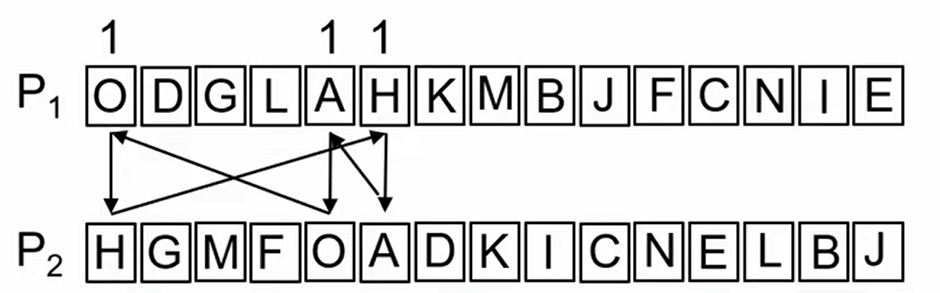
\includegraphics[width=\textwidth]{Degree//static/AI_TSP_ga_cycle1.png}
            \caption{TSP cycle 1}
        \end{subfigure}
        \hfill
        \begin{subfigure}[b]{0.45\textwidth}
            \centering
            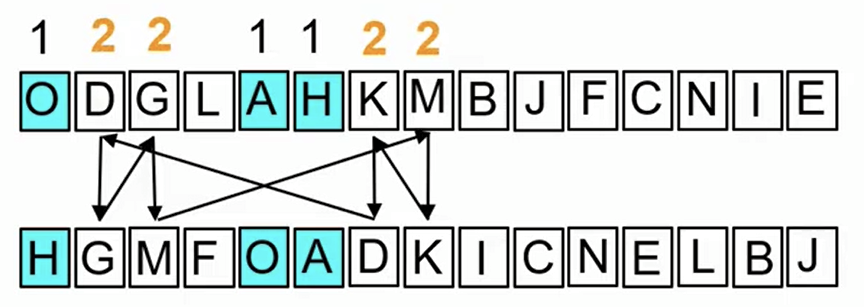
\includegraphics[width=\textwidth]{Degree//static/AI_TSP_ga_cycle2.png}
            \caption{TSP cycle 2}
        \end{subfigure}
        \caption{TSP Identifying cycles}
    \end{figure}
    Once cycles are identified, then $C_1$ gets odd numbered cycles from $P_1$ and even numbered cycles from $P_2$ the other go to $C_2$.
    \item \textbf{Partially Mapped Crossover(PMX)}: Identify some cities that form a subtour and establish a mapping.
    \begin{figure}[H]
        \centering
        \begin{subfigure}[b]{0.45\textwidth}
            \centering
            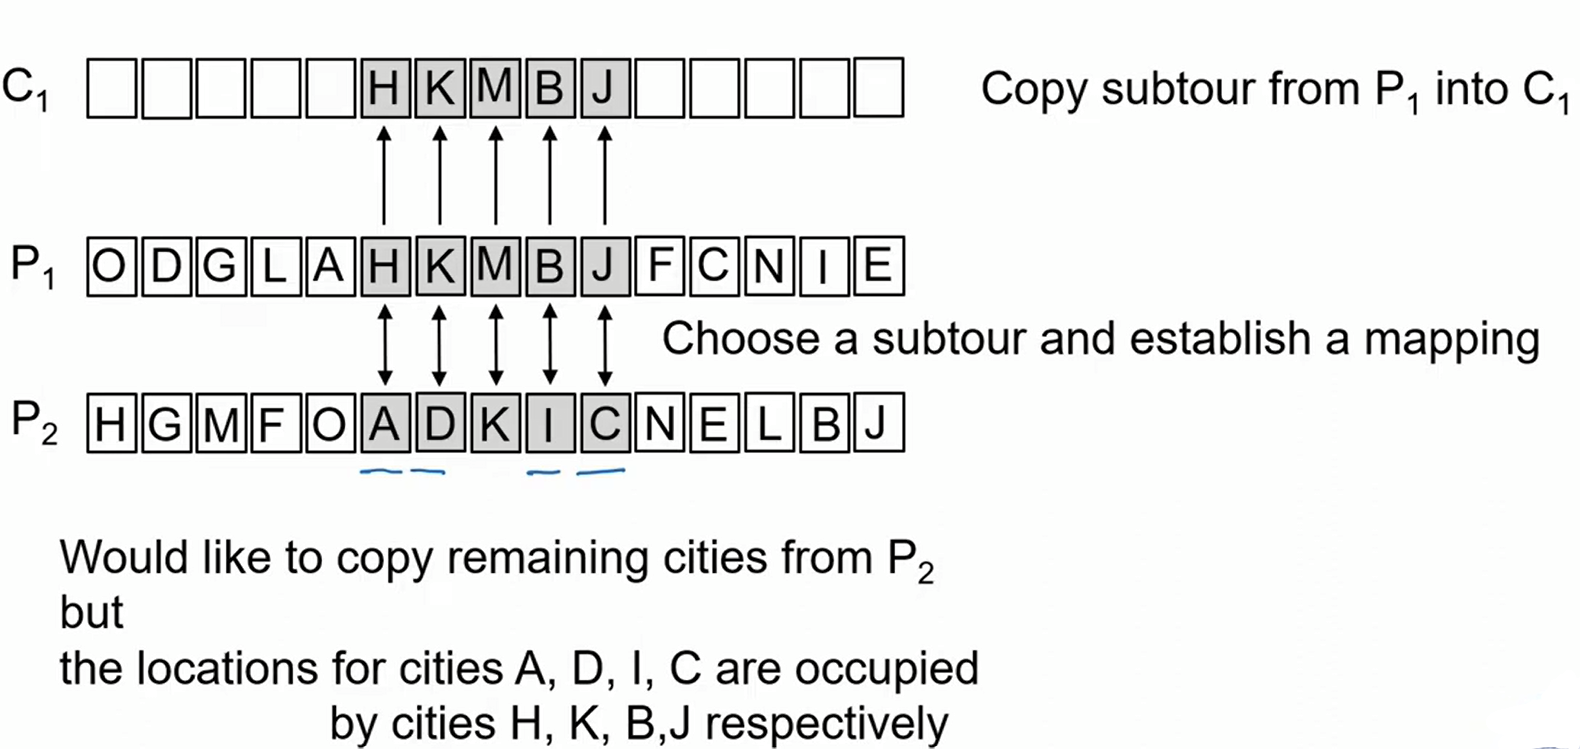
\includegraphics[width=\textwidth]{Degree/static/AI_TSP_partialcrossover_subtour.png}
            \caption{Choose Subtour}
        \end{subfigure}
        \hfill
        \begin{subfigure}[b]{0.45\textwidth}
            \centering
            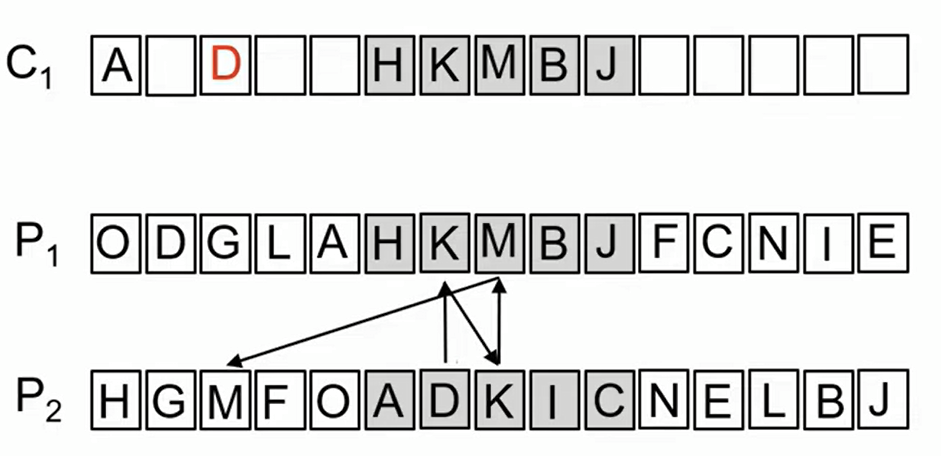
\includegraphics[width=\textwidth]{Degree/static/AI_TSP_partialcrossover_rest.png}
            \caption{Copy occupied spaces}
        \end{subfigure}
        \caption{Partially Mapped Crossover}
    \end{figure}
    \item \textbf{Order Crossover}: Copy a subtour from $P_1$ into $C_1$ and the remaining from $P_2$ in the order they occur in $P_2$.
    \item For all the above we were using path representation of TSP, there is another representation of TSP.
    \item \textbf{Adjacency Representation}: The cities are arranged based on where they come from in the tour with respect to the index. For example if $A\rightarrow H$, then at index 0 we would have $H$.
    \item \textbf{Alternating Edges Crossover}: From a given city $X$ choose the next city $Y$ from $P_1$ and from the city $Y$ choose the next city from $P_2$ and so on. It is possible to run into cycles, need to be careful.
    \item \textbf{Heuristic Crossover}: For each city choose the next from that parent $P_1$ or $P_2$ whichever is closer.
    \item \textbf{Ordinal Representation}: Replace the name of the city is Path Representation one by one to its current numeric index. At the start all cities $A,B,C,D,E$ will have numeric index $1,2,3,4,5$, now consider if we add $C$ to the representation the new indexing would be for cities $A,B,D,E$, we have $1,2,3,4$. The \textbf{advantage} is that single point crossover produces valid offspring.
\end{itemize}

\subsection{Ant Colony Optimization}
\begin{itemize}
    \item \textbf{Emergent Systems}: Collections of simple entities organize themselves and a larger more sophisticated entity emerges. The behavior of this complex system is a property that emerges from interactions amongst its components.
    \item \textbf{Conway's Game of Life}: A cellular automaton in which cells are alive or dead. Each cell obeys the following rules to decide its fate in the next time step.
    \begin{table}[H]
        \centering
        \begin{tabular}{|c|c|c|}
            \hline
            Cell state & Number of alive neighbors & New cell state \\
            \hline
            alive & $<2$ & dead \\
            \hline
            alive & 2 or 3 & alive \\
            \hline
            alive & $>3$ & dead \\
            \hline
            dead & 3 & alive \\
            \hline
        \end{tabular}
        \caption{Rules for Game of Life}
        \label{tab:AI-rules-game-life}
    \end{table}
    \item Illusion of movement can be seen in an example called \textbf{Gosper's Glider Gun}.
    \item \textbf{Chaos and Fractals}: A fractal is a never-ending pattern. Fractals are infinitely complex patterns that are self-similar across different scales. They are created by repeating a simple process over and over in an ongoing feedback loop. Drive by recursion, fractals are images of dynamic systems, the pictures of chaos.
    \item Let 5 ants $A,B,C,D,$ and $E$ go out in search for food. Each ant lays a trail of pheromone where it goes. Each ant lays a trail of pheromone where it goes. More ants that emerge will tend to follow some pheromone trail.
    \item Let's say $A$ finds some food, then it will follow its pheromone trail back and the other ants will continue their search.
    \item Eventually, as more ants travel on the trail they deposit more pheromone and the trail gets stronger and stronger, eventually becoming the caravan we might have seen raiding our food. 
    \item They tend to find the shortest path.
    \item \textbf{Ant Colony Optimization}: We try to capitalize on this method. Each ant constructs a solution using a stochastic greedy method using a combination of a heuristic function and pheromone trail following.
    \item This is related to the class of algorithms known as \textit{Swarm Optimization}.
    \begin{algorithm}[H]
        \caption{Ant Colony Optimization for TSP}\label{alg:AI-ant-colony-tsp}
        \begin{algorithmic}[1]
            \Statex \Call{TSP-ACO}{ }
            \State $bestTour\gets$ NIL
            \Repeat
                \State randomly place $M$ ants on $N$ cities
                \For{each ant $a$}
                    \For{$n\gets$ $1$ to $N$}
                        \State ant $a$ selects an edge from the distribution $P_n^a$
                    \EndFor
                \EndFor
                \State update $bestTour$
                \For{each ant $a$}
                    \For{each edge $(u,v)$ in the ant's tour}
                        \State deposit pheromone $\propto$ 1/tour-length on edge $(u,v)$
                    \EndFor
                \EndFor
            \Until{some termination criteria}
            \State \Return $bestTour$
        \end{algorithmic}
    \end{algorithm}
    \item From a city $i$ the $k^{th}$ ant moves to city $j$ with a probability given by
    \begin{equation*}
        P^k_{ij}(t)=\begin{cases}
            \frac{[\tau_{ij}(t)]^\alpha \times [\eta_{ij}]^\beta}{\sum_{h\in allowed_k(t)}([\tau_{ih}(t)]^\alpha [\eta_{ih}(t)]^\beta)},\text{ if }j\in allowed_k(t)\text{ the cities ant }k\text{ is allowed to move to}\\
            0,\text{ otherwise}
        \end{cases}
    \end{equation*}
    where $\tau_{ij}(t)$ is pheromone on edge$_{ij}$ and $\eta_{ij}$ is called visibility which is inversely proportional to the distance between cities $i$ and $j$.
    \item After constructing a tour in $n$ time steps, each ant $k$ deposits an amount of pheromone $\frac{Q}{L_k}$ on the edges it has traversed, which is inversely proportional to the cost of the tour $L_k$ it found.
    \item Total pheromone deposited on edge$_{ij}$ is $\Delta \tau_{ij}(t,t+n)$
    \item The total pheromone on edge$_{ij}$ is updated as
    \begin{equation*}
        \tau_{ij}(t+n)=(1-\rho)\times \tau_{ij}(t)+\Delta \tau_{ij}(t,t+n)
    \end{equation*}
    where $\rho$ is the rate of evaporation of pheromone.
\end{itemize}

\section{Finding Optimal TSP Tours}
\subsection{Finding Optimal Paths}
\begin{itemize}
    \item Breadth First Search finds a solution with the smallest \textit{number} of moves. But if \textit{cost} of all moves is no the same then an \textbf{optimal} solution may not be the one with the smallest number of moves.
    \item \textbf{Brute Force}: Simply search the entire search tree, computationally it is mindlessly expensive.
    \item \textbf{Goal}: Search as little of the space as possible while guaranteeing the optimal solution.
    \item A \textit{Best First} approach to solving problems. Given a set of candidates a search algorithm has to choose from. Each candidate is tagged with an estimated cost of the complete solution.
    \item Branch and Bound in a refinement space
    \begin{enumerate}
        \item Initial solution set contains all solutions.
        \item In each step we partition a set into two smaller sets.
        \item Until we can pick a solution that is fully specified.
        \item Each solution set needs to have an estimated cost.
        \item B\&B will refine the solution that has the least estimated cost.
    \end{enumerate}
    \item An optimal solution can be guaranteed by ensuring that the estimated cost is a lower bound on actual cost.
    \item \textbf{Lower bound}: A solution will never be cheaper than it is estimated to be.
    \item Thus if a fully refined solution is cheaper than a partially refined one, the latter need not be explored - \textbf{PRUNING}. The higher the estimate, the better the pruning.
    \item Branch and Bound for TSP
    \begin{enumerate}
        \item Let the candidate solutions be permutations of the list of city names.
        \item The initial set of candidates includes all permutations.
        \item Refine the cheapest set by specifying a specific segment.
        \item Heuristic: Choose the segment with minimum cost.
        \item For tighter estimates, edges that cause three or more segment cycles are avoided.
        \item We, can also exclude an edge that is a third edge for a node, because a city has only two neighbors in a tour.
        \item Higher estimates require more work.
    \end{enumerate}
    \item A lower bound estimate could be for each row add up the smallest two positive entries and divide by two. This may not feasible.
    \item The basic idea behind B\&B is to prune those parts of a search space which cannot contain a better solution.
    \item Each candidate is tagged with an estimated cost of the complete solution.
    \item \textbf{Dijkstra's Algorithm}
    \begin{enumerate}
        \item Begins by assigning infinite cost estimates to all nodes except the start node.
        \item It assigns color white to all the nodes initially.
        \item It picks the cheapest white node and colors it black.
        \item \textbf{Relaxation}: Inspect all neighbors of the new black node and check if a cheaper path has been found to them.
        \item If yes, then update cost of that node, and mark the  parent node.
    \end{enumerate}
\end{itemize}

\subsection{Algorithm A*}
\begin{itemize}
    \item A* achieves better performance by using heuristics to guide its search.
    \item For all nodes we will compute $f(n)$ which is made up of two components $g(n)$ and $h(n)$.
    \item $g(n)$ = actual cost of solution found from the start node to node $n$.
    \item $h(n)$ = estimated cost of the path from node $n$ to goal node.
    \item Maintain a priority queue of nodes sorted on the $f$ values
    \item Pick the lowest $f$ value node, and check whether it is the goal node.
    \item Else generate its neighbors, and compute their $f$ values
    \item Insert new nodes into the priority queue
    \item For existing nodes check for better path(like Dijkstra's algorithm)
    \begin{algorithm}[H]
        \caption{A* Algorithm}\label{alg:AI-A*}
        \begin{algorithmic}[1]
            \Statex \Call{A*}{S}
            \State default value of $g$ for every node is $+\infty$
            \State $parent(S)\gets null$
            \State $g(S)\gets 0$
            \State $f(S)\gets g(S)+h(S)$
            \State $OPEN\gets$ $S:$[ ]
            \State $CLOSED\gets$ empty list
            \While{$OPEN$ is not empty}
                \State $N\gets$ remove node with the lowest $f$ value from $OPEN$
                \State add $N$ to CLOSED
                \If{\Call{GoalTest}{$N$}}
                    \State \Return \Call{ReconstructPath}{$N$}
                \EndIf
                \For{each neighbor $M\in $ \Call{MoveGen}{$N$}}
                    \If{$g(N)+k(N,M)<g(M)$}
                        \State $parent(M)\gets N$
                        \State $g(M)\gets g(N)+k(N,M)$
                        \State $f(M)\gets g(M)+h(M)$
                        \If{$M\in OPEN$} 
                            \State continue 
                        \EndIf
                        \If{$M\in CLOSED$} 
                            \State \Call{Propagate-Improvement}{$M$}
                        \Else 
                            \State add $M$ to $OPEN$ 
                        \EndIf
                    \EndIf
                \EndFor
            \EndWhile
            \Return empty list
        \end{algorithmic}
    \end{algorithm}
    \item Propagate improvement simply does line 13 to 17 recursively.
    \item A* is admissible if
    \begin{enumerate}
        \item The branching factor is finite, otherwise you cannot even generate the neighbors.
        \item Every edge has a cost greater than a small constant $\epsilon$, however it is possible to get stuck in an infinite path with a finite cost.
        \item For all nodes $h(n)\leq h*(n)$
    \end{enumerate}
    \item If a path exists to the goal node, then the OPEN list always contains a node $n'$ from an optimal path. Moreover, the $f$ value of that node is not greater than the optimal value.
\end{itemize}

\end{document}